\documentclass{beamer}

\usetheme{metropolis}
\usepackage{appendixnumberbeamer}

\usepackage{transparent}
\usepackage[english]{babel}
\usepackage[sfdefault]{FiraSans}
\usepackage{amssymb,mathrsfs,mathtools}
\usepackage{amsfonts}
\usepackage{tikz,pgfopts,etoolbox,calc,ifxetex,ifluatex}
\usefonttheme[onlymath]{serif}

\setbeamercovered{highly dynamic}

\title{\textsc{A Bayesian model for data flow: BikeMi}}
\subtitle{}
\author{Andrea De Gobbis, Lorenzo Ghilotti, Giorgio Meretti}
\institute{Politecnico di Milano}
\logo{\includegraphics[width=15mm]{Politecnico_di_Milano}}
\date{January 8, 2020}
\usetheme{Goettingen}
\usecolortheme{dolphin}

\begin{document}
\begin{frame}
	\maketitle	
\end{frame}

\begin{frame}{What we are doing}

The BikeMi stations net in Milan
\begin{figure}[H]
\centering
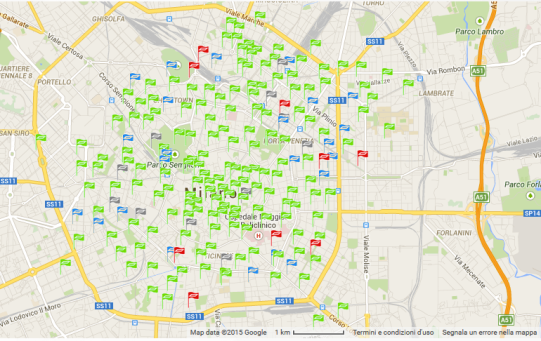
\includegraphics[width=1\linewidth]{pictures/mappa.png} 
\end{figure}

\end{frame}


\begin{frame}{Two prospective of the problem}

We followed two distinct paths:

\vspace{5mm}

\begin{columns}

\begin{column}{.5\textwidth}

	\alert{Global model:} the total volume of bikes travels in a specific day $Y_t$ without considering the graph structure. This results in a single time series.

\end{column}

\hspace{5pt}

\vrule{}

\hspace{8pt}

\begin{column}{.5\textwidth}
	\transparent{0.5}
	{
	\alert{Network model:} dividing in the different nodes and analysing the flow of bikes in the net. The dimensionality is much higher.
	}

\end{column}

\end{columns}

\end{frame}

\begin{frame}{Poisson model}

Day by day \alert{Poisson}:
\begin{equation}
\begin{cases}
Y_t \sim \mathrm{Po}(Y_t|\lambda_t) \\
\lambda_t = \exp\{\alpha + \boldsymbol{\beta}\cdot \mathbf{x}_t\}\\
\alpha \sim \mathcal{N}(0,\sigma^2_\alpha)\\
\beta_i \overset{iid}{\sim}\mathcal{N}(0,\sigma^2_\beta)
\end{cases}
\end{equation}
\end{frame}

\begin{frame}{Poisson model}

With \alert{covariates} $\mathbf{x}_{t}$:

\begin{itemize}

	\item $Y_{t-1}$ volume on the previous day

	\item $Y_{t-7}$ volume on the same weekday of the previous week

	\item $W_t$ dummy for weekday / weekend

	\item $R_t, R_{t-1}$ dummies for rain in the current and previous day

	\item $T_t$ mean temperature for the day

	\item $S_t, M_t$ dummies for Saturday and Monday 

\end{itemize}

\end{frame}


\begin{frame}{Predictive distribution of the poisson model}

Only 3 of 35 in the 90\% credible interval

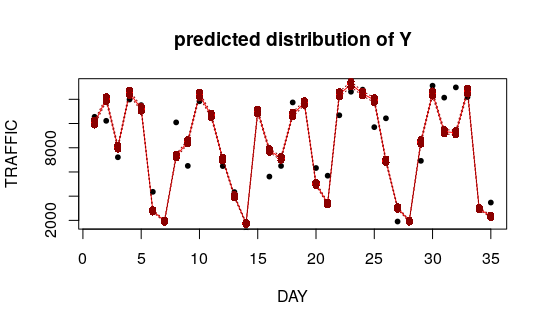
\includegraphics[width=0.95\linewidth]{pictures/poiss_pred.png} 

\end{frame}
	
\begin{frame}{Time series model: BSTS}
\begin{equation}
\begin{cases}
\mathbf{X}(t) = \mathbf{f}(\mathbf{X}(1:(t-1))) +  \boldsymbol{\epsilon}_1(t)\\
\mathbf{Y}(t) = \mathbf{g}(\mathbf{X}(t)) +  \boldsymbol{\epsilon}_2(t)
\end{cases}
\end{equation}

with \alert{suitable initial conditions and priors}
\end{frame}

\begin{frame}{Time series model: BSTS}
\alert{Elementary model} with precisions
\begin{equation}
\begin{cases}
Y_t = \mu_t + \gamma_t + \frac{1}{\sqrt{\tau_\epsilon}}\tilde{\epsilon}_t\\
\\
\mu_t = \mu_{t-1} + \delta_{t-1}+ \frac{1}{\sqrt{\tau_\eta}}\tilde{\eta}_t\\
\delta_t = \delta_{t-1} + \frac{1}{\sqrt{\tau_v}}\tilde{v}_t\\
\gamma_t = \sum_{i=1}^{S-1}\gamma_{t+i-S} + \frac{1}{\sqrt{\tau_w}}\tilde{w}_t\\
\\
\tilde{\epsilon}_t, \tilde{\eta}_t, \tilde{v}_t, \tilde{w}_t, \overset{iid}{\sim} \mathcal{N}(0,1)\\
\end{cases}
\end{equation}
\end{frame}

\begin{frame}{Time series model: BSTS}
Elementary model priors
\begin{equation}
\begin{cases}
\mu_0 \sim \mathcal{N}(m, \tau_m)\\
\delta_0 \sim \mathcal{N}(d, \tau_d)\\
\boldsymbol{\gamma}_{0:(2-S)} \sim \mathcal{N}_{S-1}(\mathbf{g}, \tau_g\mathbf{I})\\
\\
\tau_* \sim Gamma(a_*, b_*),\ with\ *=\{\epsilon, \eta, v,w\}\\
\\

\{\tilde{\epsilon}_t, \tilde{\eta}_t, \tilde{v}_t, \tilde{w}_t, \mu_0, \delta_0, \boldsymbol{\gamma}_{0:(-S+2)}, \tau_\epsilon, \tau_\eta, \tau_v, \tau_w\}\\
independent.
\end{cases}
\end{equation}
\end{frame}

\begin{frame}{Time series model: BSTS}
\alert{Complete model} with precisions
\begin{equation}
\begin{cases}
Y_t = \mu_t + \gamma_t + \rho_t + \boldsymbol{\beta}^T\mathbf{z}_t + \frac{1}{\sqrt{\tau_\epsilon}}\tilde{\epsilon}_t\\
\\
\mu_t = \mu_{t-1} + \delta_{t-1} +\frac{1}{\sqrt{\tau_\eta}}\tilde{\eta}_t\\
\delta_t = \delta_{t-1} + \frac{1}{\sqrt{\tau_v}}\tilde{v}_t\\
\gamma_t = \sum_{i=1}^{S-1}\gamma_{t+i-S} + \frac{1}{\sqrt{\tau_w}}\tilde{w}_t\\
\rho_t = \alpha\rho_{t-1} + \frac{1}{\sqrt{\tau_u}}\tilde{u}_t\\
\\
\tilde{\epsilon}_t, \tilde{\eta}_t, \tilde{v}_t, \tilde{w}_t, \tilde{u}_t \overset{iid}{\sim} \mathcal{N}(0,1)\\
\end{cases}
\end{equation}
\end{frame}

\begin{frame}{Time series model: BSTS}
Complete model priors
\begin{equation}
\begin{cases}
\mu_0 \sim \mathcal{N}(m, \tau_m)\\
\delta_0 \sim \mathcal{N}(d, \tau_d)\\
\boldsymbol{\gamma}_{0:(2-S)} \sim \mathcal{N}_{S-1}(\mathbf{g}, \tau_g\mathbf{I})\\
\rho_0 \sim \mathcal{N}(r, \tau_r)\\
\boldsymbol{\beta} \sim \mathcal{N}_p(\mathbf{0}, \tau_b \mathbf{I})\\
\alpha \sim \mathcal{N}(a, \tau_a)\\
\tau_* \sim Gamma(a_*, b_*),\ with\ *=\{\epsilon, \eta, v,w,u\}\\
\{\tilde{\epsilon}_t, \tilde{\eta}_t, \tilde{u}_t, \tilde{w}_t, \tilde{v}_t, \mu_0, \delta_0, \boldsymbol{\gamma}_{0:(-S+2)}, \rho_0\, \boldsymbol{\beta}, \alpha, \tau_\epsilon, \tau_\eta, \tau_v, \tau_w, \tau_u\}\\ independent .
\end{cases}
\end{equation}
\end{frame}

\begin{frame}{Time series model: BSTS}
\alert{Robust model} with precisions
\begin{equation}
\begin{cases}
Y_t = \mu_t + \gamma_t + \rho_t + \boldsymbol{\beta}^T\mathbf{z}_t + \frac{1}{\sqrt{\tau_\epsilon}}\tilde{\epsilon}_t\\
\\
\mu_t = avgpred(\mu_t) + avgpred(\delta_t) +\frac{1}{\sqrt{\tau_\eta}}\tilde{\eta}_t\\
\delta_t = avgpred(\delta_t) + \frac{1}{\sqrt{\tau_v}}\tilde{v}_t\\
\gamma_t = \sum_{i=1}^{S-1}\gamma_{t+i-S} + \frac{1}{\sqrt{\tau_w}}\tilde{w}_t\\
\rho_t = \alpha\rho_{t-1} + \frac{1}{\sqrt{\tau_u}}\tilde{u}_t\\
\\
\tilde{\epsilon}_t, \tilde{\eta}_t, \tilde{v}_t, \tilde{w}_t, \tilde{u}_t \overset{iid}{\sim} \mathcal{N}(0,1)\\
\end{cases}
\end{equation}

where  $ avgpred(\phi_t) =\frac{1}{2}\phi_{t-1} + \frac{1}{3}\phi_{t-S} + \frac{1}{6} \phi_{t-2S}$\\
and same priors as before
\end{frame}

\begin{frame}{Time series model: BSTS}
\alert{Instability} of the errors, $ \tau_\epsilon $ explodes, bad autocorrelation
\begin{figure}[H]
	\centering
	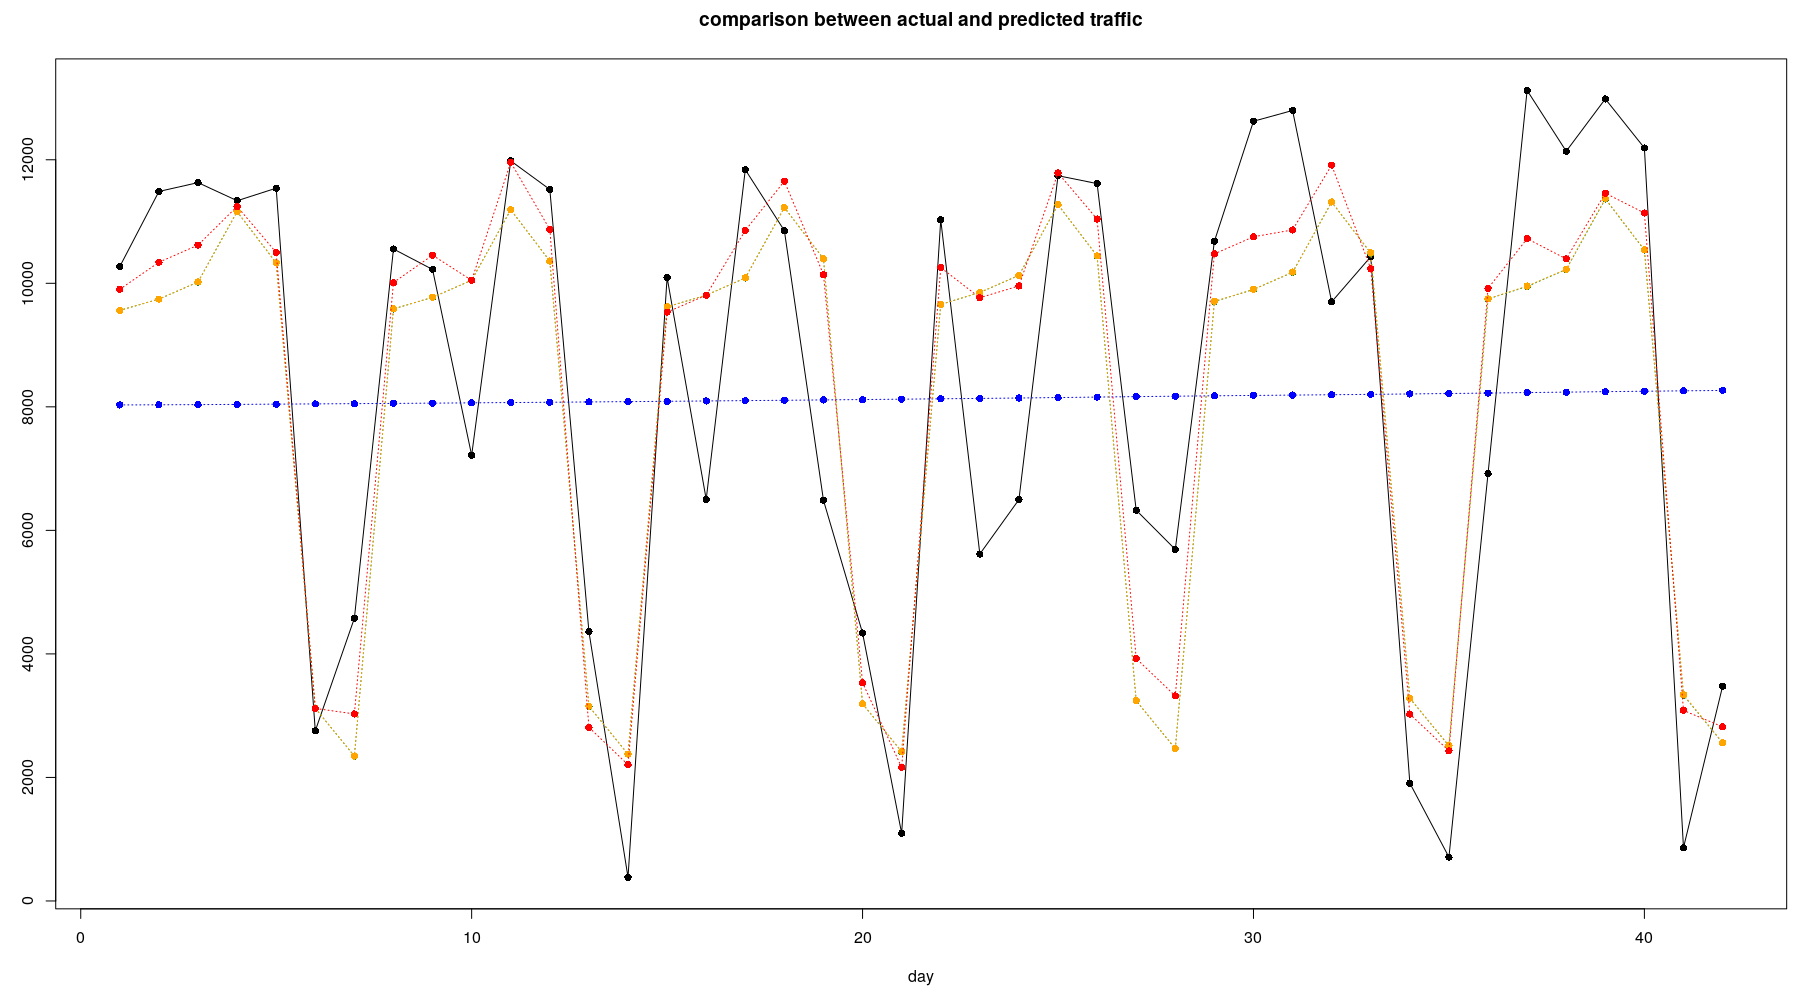
\includegraphics[width=1\linewidth]{pictures/erratic.png} 
	\label{fig1}
\end{figure}

\end{frame}

\begin{frame}{Time series model: BSTS}
\alert{Instability} of the errors, $ \tau_\epsilon $ explodes, bad autocorrelation
\begin{figure}[H]
	\centering
	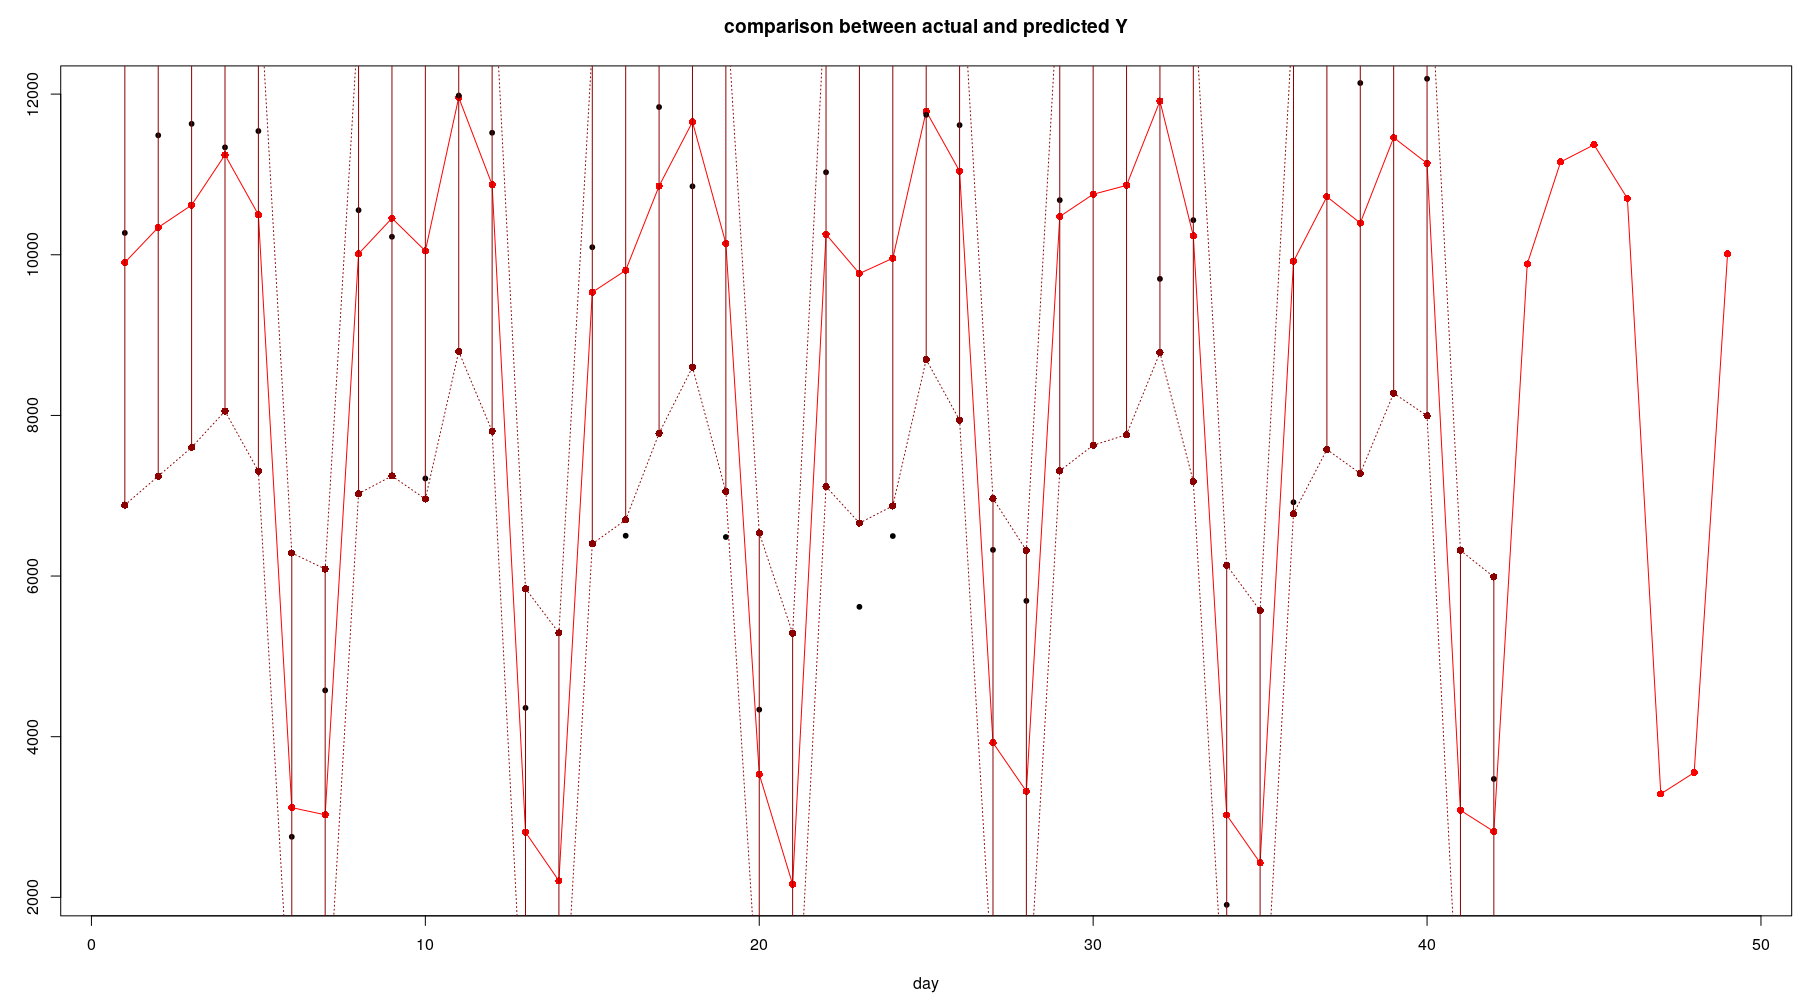
\includegraphics[width=1\linewidth]{pictures/erratic2.png} 
	\label{fig2}
\end{figure}

\end{frame}

\begin{frame}{Time series model: BSTS}
\alert{Blocking} the maximum variance, $ \tau_* $ under control, partial mixing of state variables
\begin{figure}[H]
	\centering
	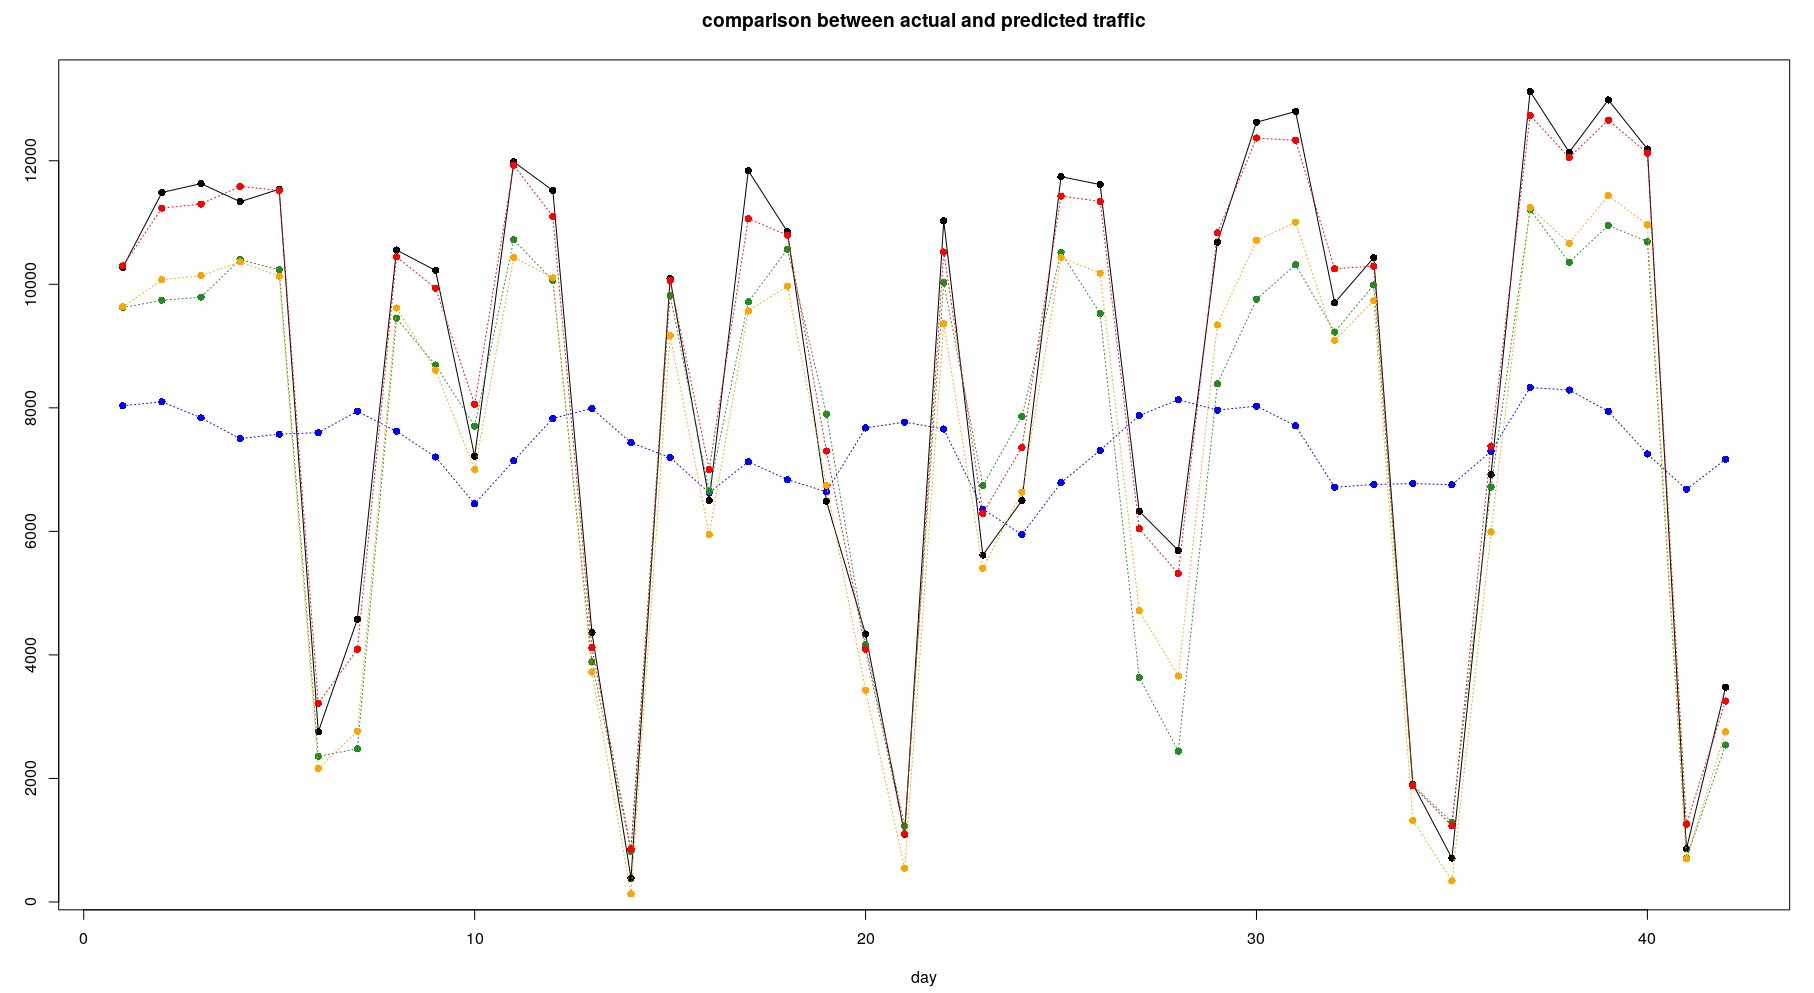
\includegraphics[width=1\linewidth]{pictures/good.png} 
	\label{fig3}
\end{figure}
\end{frame}

\begin{frame}{Time series model: BSTS}
Smaller induced variability, \alert{attempt of prediction} with real weather.
\begin{figure}[H]
	\centering
	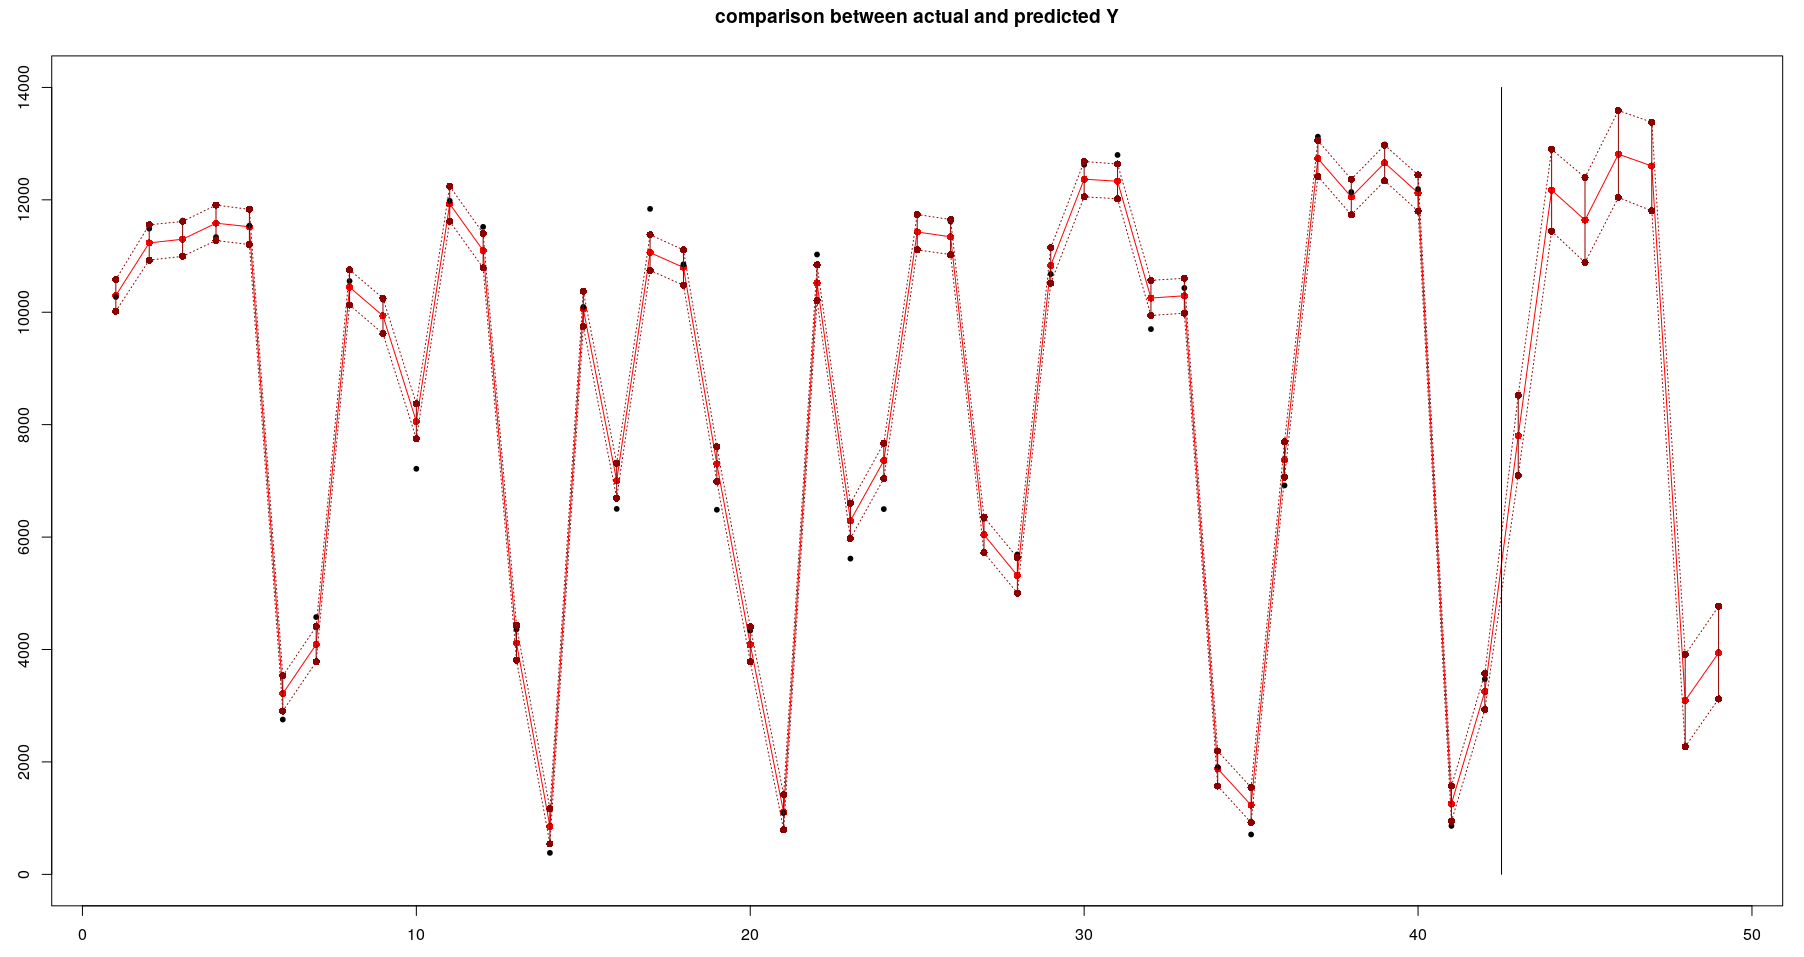
\includegraphics[width=1\linewidth]{pictures/good2.png} 
	\label{fig4}
\end{figure}

\end{frame}

\begin{frame}{Time series model: BSTS}
\alert{Comparison} truncated-variance robust BSTS vs Poisson.

Observations inside \alert{credibility intervals}:
\begin{itemize}
	\item Poisson 3/35
	\item BSTS 24/42
\end{itemize} 

\alert{WAIC}:
\begin{itemize}
	\item Poisson -0.0171
	\item BSTS -0.0160
\end{itemize} 

\end{frame}


\begin{frame}{Time series model: BSTS}
\alert{Robust model for time zones} with precisions
\begin{equation}
\begin{cases}
Y_{th} = \mu_t + \gamma_t + \rho_t + \chi_k + \boldsymbol{\beta}^T\mathbf{z}_t + \frac{1}{\sqrt{\tau_\epsilon}}\tilde{\epsilon}_{th}\\
\\
\mu_t = avgpred(\mu_t) + avgpred(\delta_t) +\frac{1}{\sqrt{\tau_\eta}}\tilde{\eta}_t\\
\delta_t = avgpred(\delta_t) + \frac{1}{\sqrt{\tau_v}}\tilde{v}_t\\
\gamma_t = \sum_{i=1}^{S-1}\gamma_{t+i-S} + \frac{1}{\sqrt{\tau_w}}\tilde{w}_t\\
\rho_t = \alpha\rho_{t-1} + \frac{1}{\sqrt{\tau_u}}\tilde{u}_t\\
\chi_k = \sum_{i=1}^{F-1}\chi_{k+i-F} + \xi\delta_{t(k)=6,7} + \frac{1}{\sqrt{\tau_\zeta}}\tilde{\zeta}\\
\\
\tilde{\epsilon}_t, \tilde{\eta}_t, \tilde{v}_t, \tilde{w}_t, \tilde{u}_t, \tilde{\zeta} \overset{iid}{\sim} \mathcal{N}(0,1)\\
\end{cases}
\end{equation}

where  $ avgpred(\phi_t) =\frac{1}{2}\phi_{t-1} + \frac{1}{3}\phi_{t-S} + \frac{1}{6} \phi_{t-2S}$, $ h=$\\$mod(k,4)+1 $
and \alert{priors of the same class as before}
\end{frame}

\begin{frame}{Time series model: BSTS}
Robust truncated variance model for time zones
\begin{figure}[H]
	\centering
	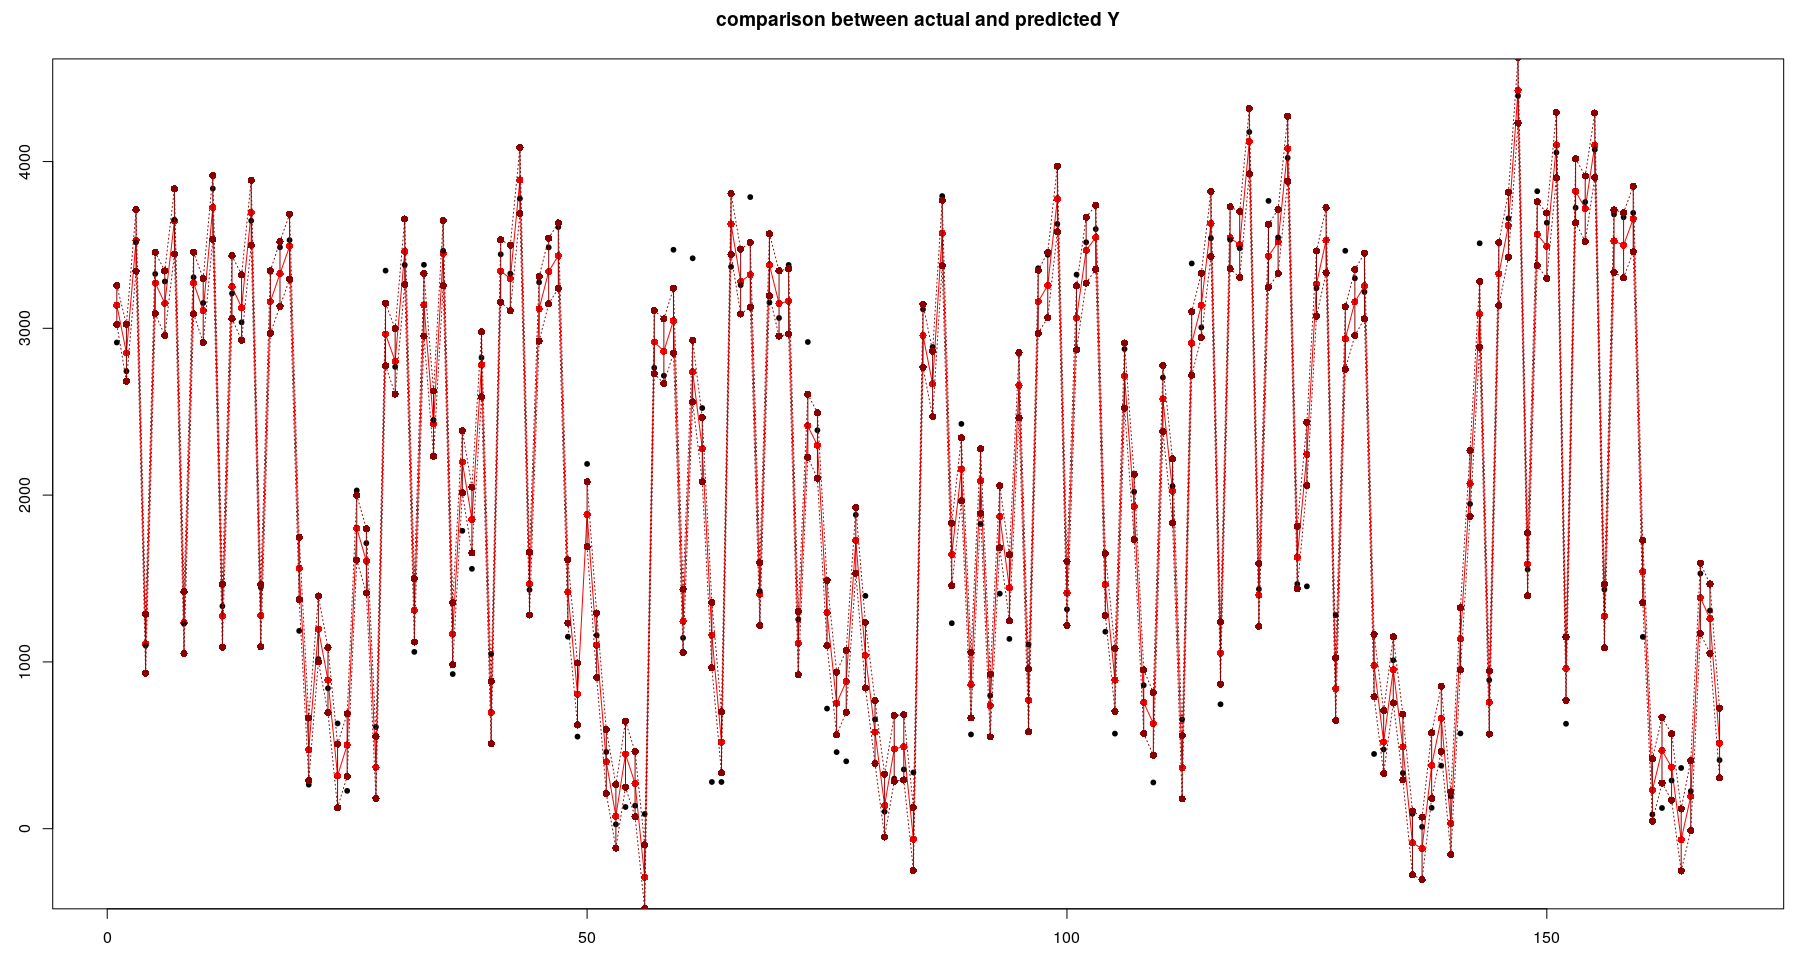
\includegraphics[width=1\linewidth]{pictures/multiple.png} 
	\label{fig5}
\end{figure}

\end{frame}

\begin{frame}{Two prospective of the problem}

We followed two distinct paths:

\vspace{5mm}

\begin{columns}
	
	\begin{column}{.5\textwidth}
		\transparent{0.5}
		{
			\alert{Global model:} the total volume of bikes travels in a specific day $Y_t$ without considering the graph structure. This results in a single time series.
		}
		
	\end{column}
	
	\hspace{5pt}
	
	\vrule{}
	
	\hspace{8pt}
	
	\begin{column}{.5\textwidth}
		\alert{Network model:} dividing in the different nodes and analysing the flow of bikes in the net. The dimensionality is much higher.
		
		
	\end{column}
	
\end{columns}

\end{frame}
\begin{frame}{Network model}

For every $(i,j)$ edge of the graph and $t \in 1:42$ we have $Y_{ij}(t)$ the number of travels from node $i$ to $j$ at day $t$.

\vspace{8mm}


\alert{Problem:}\\ more than 4 million variables $\Rightarrow$\\ \hspace{6mm}Computationally untreatable

\vspace{5mm}


\alert{Solutions:}

\begin{itemize}

\item clusterization through DBSCAN

\item simplification of the variables

\end{itemize}
\end{frame}
\begin{frame}{Preprocessing clusterization with DBSCAN}

Algorithm to divide the nodes into initial clusters. We introduced a modified version with a weight to break up the \alert{bigger clusters}, minimizing the \alert{autorings} presence.


\begin{figure}[H]


		\centering

		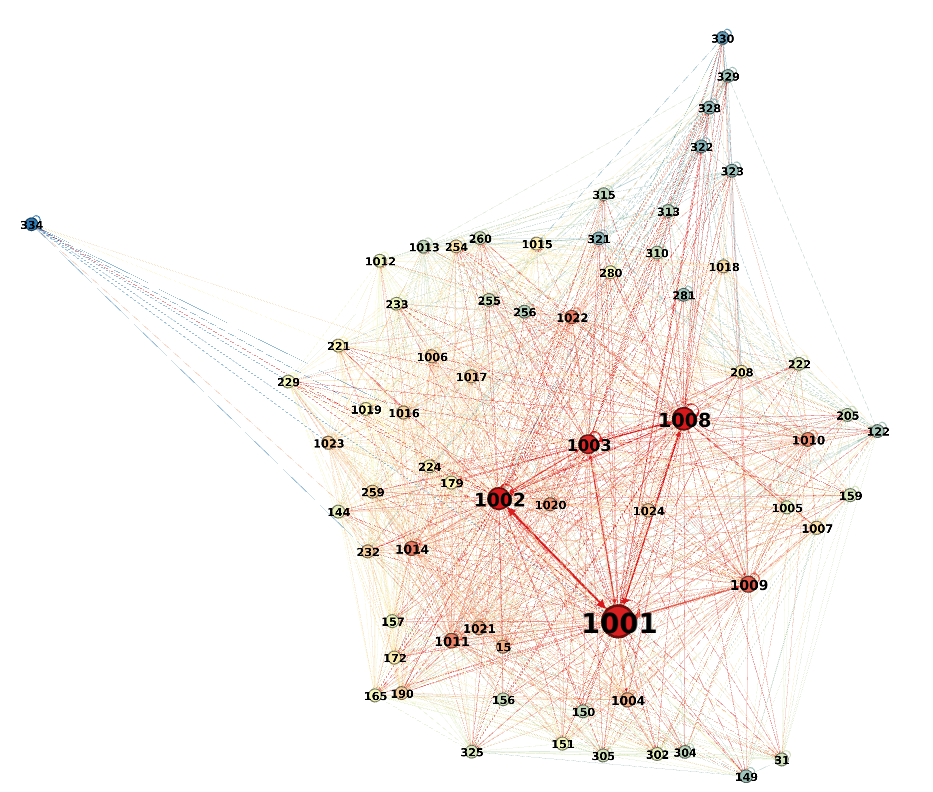
\includegraphics[width=70 mm]{pictures/old_model_gephi.png}

\end{figure}

\end{frame}

\begin{frame}
From \alert{334} nodes to \alert{140}.
	\centering

	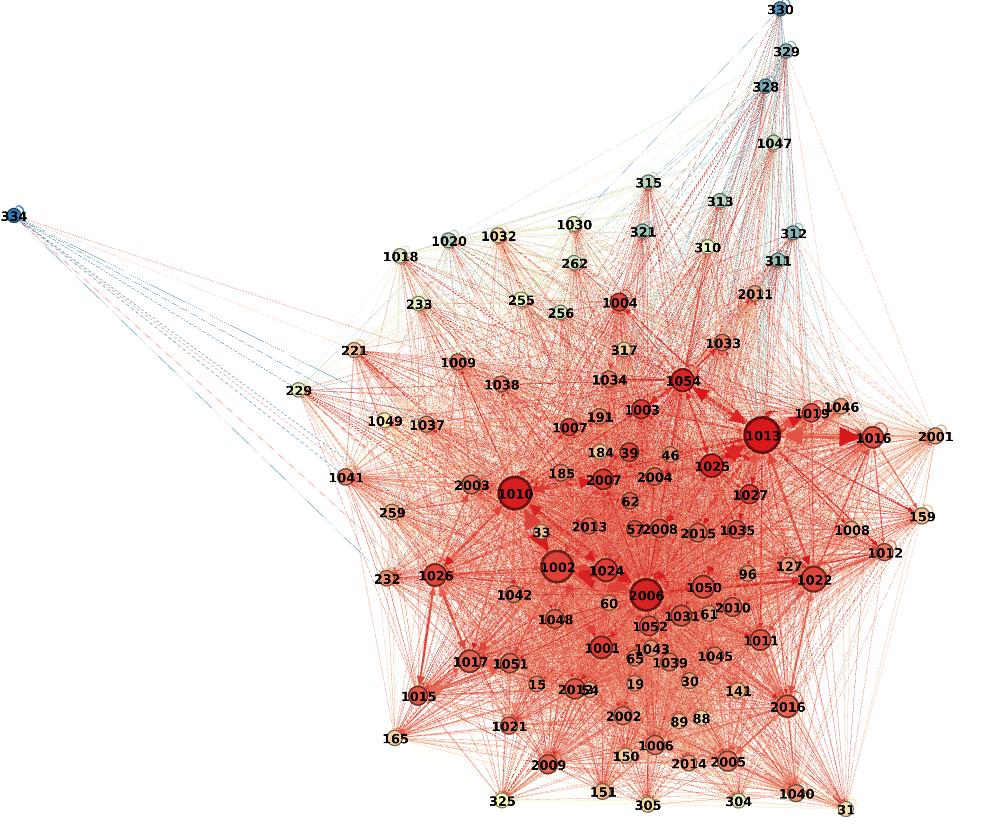
\includegraphics[width=100 mm]{pictures/new_model_gephi.png}

\end{frame}



\begin{frame}{Modeling the flux}

To further simplify the analysis we focus on the bikes arriving and departing from each node $N_i^{IN}(\Delta t)$ and $N_i^{OUT}(\Delta t)$ in the time interval $\Delta t$.

\vspace{5mm}

We are interested in the smallest $\Delta t$ as possible but this would increase the number of variables $\Rightarrow$ consider them as \alert{functional data}.

\centering
		$$V_i(t) = \lim_{\Delta t \to 0} \frac{N_i^{IN}(\Delta t) - N_i^{OUT}(\Delta t)}{\Delta t}$$

$$\Phi_i(t) = \int_{0}^{t}V_i(u)\,\mathrm{d}u$$

\end{frame}

\begin{frame}
We can analyse \alert{when new bikes should be brought to which station}.

		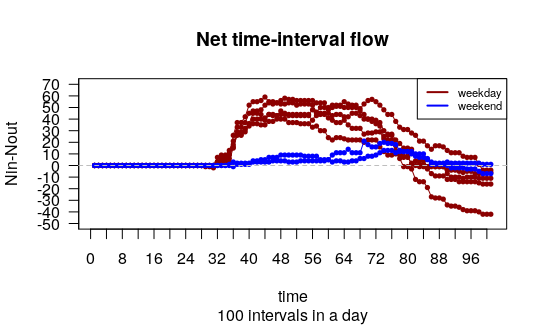
\includegraphics[width=1\textwidth]{pictures/flux.png} 

\end{frame}

\end{document}

